\documentclass{article}

\usepackage[latin1]{inputenc}
\usepackage{color}
\usepackage{listings}
\usepackage[english]{babel}
\usepackage{graphicx}
\usepackage{indentfirst}

%\usepackage{fontspec}
%\usepackage[utf8]{inputenc}
%\setmainfont{Futura}[ItalicFont={Futura Italic}]

\definecolor{colKeys}{rgb}{0,0,1}
\definecolor{colIdentifier}{rgb}{0,0,0}
\definecolor{colComments}{rgb}{0,0.5,1}
\definecolor{colString}{rgb}{0.6,0.1,0.1}

\lstset{%configuration de listings
float=hbp,
basicstyle=\ttfamily\small, 
identifierstyle=\color{colIdentifier}, 
keywordstyle=\color{colKeys}, 
stringstyle=\color{colString}, 
commentstyle=\color{colComments}, 
columns=flexible, 
tabsize=2, 
%frame=trBL, 
frameround=tttt, 
extendedchars=true, 
showspaces=false, 
showstringspaces=false, 
numbers=left, 
numberstyle=\tiny, 
breaklines=true, 
breakautoindent=true, 
captionpos=b,
xrightmargin= 1cm, 
xleftmargin= 1cm
} 
\lstset{language=c++}
\lstset{commentstyle=\textit}

\parskip 5pt plus 2pt minus 2pt
\textwidth=14cm
\oddsidemargin=1cm
\evensidemargin=1cm
\topmargin=-0.5cm
\headheight=0cm
\headsep=1cm
\textheight=23cm
\parindent=1.5cm

\begin{document}
\thispagestyle{empty}
\begin{center}
\large\bf Machine Learning Project 1 Report by Jared Manning and Egan Sutherland
\end{center}
\bigskip


\section*{1. Introduction}

\noindent In this project, we were asked to implement training and testing functions for binary decision trees. The following will describe in detail the implementation of the required and supporting methods. First, supporting classes will be described then each required function's implementation will be described. After implementation details, there will be a section for results.

\section*{2. Implementation Details}

\noindent \textbf{Class Details}

\noindent "DTree"

\indent Description: The DTree class defines objects of type DTree. This class is the Decision Tree class that is returned by each of the required training functions. In trees of this type, values of 0 of the current feature branch to the left and values of 1 branch to the right. Our diagrams follow this convention as well.

\indent Data Members:

\indent \textbullet "root" - Holds the root node of the tree. This is of type Node.

\indent \textbullet "means" - A list to hold the mean values of features when training on real-valued data. This is initialized as an empty list and is populated only when training on real-valued data sets with binary labels.

\indent Methods

\indent \textbullet Constructor - The constructor for this class initializes "root" as an empty instance of "Node" and "means" as a null pointer using the "None" keyword.

\indent \textbullet "predict(x)" - Makes a prediction based on a tree that has already been built. It takes a single sample's data and makes a prediction based on that data by calling "search" on the root, a method of the class Node, which will be described in detail later.

\indent \textbullet "build(X,Y,max\textunderscore depth)" - Takes a feature numpy array, a label numpy array, and a maximum tree depth as inputs. It then calls "split", a method of "Node" which is described later, to recursively build a decision tree. 

\indent \textbullet "toString()" - This is a function used for testing and debugging. It calls "toString", a member method of "Node" which is described later, on the root.

\indent \textbullet "fixData(X)" - This method takes real-valued input data as a numpy array or list and converts it to binary data. This method uses a nested for loop to move through each feature and each sample in the data. The "means" list contains the mean value of each feature. Each data point is checked against the corresponding feature mean. If the data point is greater than the mean, it is replaced with a value of 1. If it is less than or equal to the mean, the data point is replaced with 0. This turns all the real-valued data passed to it into binary data and returns the updated data. 

\pagebreak

\noindent "Node"

\indent Description: This class is the node used to create DTrees. One instance of "Node" is used as the root in an instance of the "DTree" class. 

\indent Data Members:

\indent \textbullet "left" - Pointer to the left child "Node".

\indent \textbullet "right" - Pointer to the right child "Node".

\indent \textbullet "feat" - At each "Node" in the "DTree", if a split is made, the index of the feature that is being used to make the split is stored in "feat". If a prediction is made at a "Node", "feat" stores "None".

\indent \textbullet "label" - This stores a binary value based on the best prediction that could be made at that node in the decision tree. Each "Node" instance stores a value in "label" but is only checked if at a leaf in the tree.

\indent \textbullet "depth" - This stores the level of the "Node" in the "DTree". The "root" of a "DTree" has a depth of 0.

\indent Methods

\indent \textbullet "search(x)" - This method takes a single sample of feature data and returns a prediction based on that data. The method checks if the current "Node" is a leaf and returns "label" if it is. Otherwise it compares the current "feat" to the sample and makes a recursive call to the right child if the feature value of the sample is nonzero or to the left child if the feature value of the sample is 0.

\indent \textbullet "split(X,Y,max\textunderscore depth)" - It is a recursive function that takes sample features, sample labels, and max\textunderscore depth as parameters. It first assigns a label to the node based on the majority of the sample labels passed in. It then checks for the base cases of either reaching the max\textunderscore depth or running best\textunderscore IG and finding and it returning "None". If not at the base case, it splits the samples based on the feature returned by best\textunderscore IG, and then recurses on the left child with all the samples that are a 0 for that feature going to the left child and then does the same for the right child.

\indent \textbullet "toString()" - This method was created for debugging purposes and is not called by any provided methods or functions. It performs a pre-order traversal of the tree, printing feature, label, and depth information at each node.

\noindent \textbf{Helper Function Details}

\noindent "best\textunderscore IG(X,Y)" - 

\indent Parameters and Returns: X is a 2D array of samples feature information and Y is a 2D array of samples label information. This function returns an integer representing the feature index that gives the maximum information gain when split on, or None if information gain is 0 for all features.

\indent Description: First, it calculates the entropy of the entire dataset (X,Y). Then, it iterates through each feature in X, splitting on it then finding the entropy of the left and right side and uses that to calculate the information gain. After going through each feature, it chooses the feature that gave the maximum information gain and returns that index, unless they were all zero in which case it returns "None".

\noindent "findMeans(X)" 

\indent Parameters and Returns: This function takes a numpy array of feature data as input and returns a list containing the mean value of each feature.

\indent Description: This function finds the number of samples and number of features. Then for each feature, it totals the values of the samples then divides that by the number of samples. It then appends it to a list of means. Each entry in the list corresponds to the mean value of a particular feature.

\noindent \textbf{Required Function Details}

\noindent "DT\textunderscore train\textunderscore binary(X,Y,max\textunderscore depth)"

\indent Parameters and Returns: "X" is a 2D numpy array containing feature data for a set of samples. "Y" is a numpy array containing the corresponding label data. "max\textunderscore depth" is the maximum depth of tree that this function can build. If -1 is passed here the tree will be built without a maximum depth and will finish when its information gain hits 0.

\indent Description: This function instantiates a "DTree" object then calls its "build()" method, passing X, Y, and max\textunderscore depth as parameters. "build()" returns a DTree, which is then returned by this function.

\noindent "DT\textunderscore test\textunderscore binary(X,Y,DT)"

\indent Parameters and Returns: "X" is a 2D numpy array containing feature data, "Y" is a numpy array containing the corresponding labels, and "DT" is a decision tree that has already been created and trained. This function returns a scalar value representing the accuracy of predictions made by "DT" on "X" and "Y".

\indent Description: This function iterates through all the samples in "X", running "predict()" on each sample. Each prediction is then compared with corresponding value in "Y". If the prediction is correct a counter is incremented. Accuracy is then calculated by dividing the counter's value by the number of samples. That accuracy value is then returned.

\noindent "DT\textunderscore train\textunderscore binary\textunderscore best(X\textunderscore train, Y\textunderscore train, X\textunderscore val, Y\textunderscore val)"

\indent Parameters and Returns: "X\textunderscore train" and "Y\textunderscore train" comprise the training data and corresponding labels. "X\textunderscore val" and "Y\textunderscore val" comprise the validation data and corresponding labels. This function returns the most accurate "DTree" it created.

\indent Description: First, this function instantiates a pointer called forest that will hold a list of all the "DTree" objects created in this function. A for loop then adds a "DTree" to the list for each feature and trains it using "X\textunderscore train" and "Y\textunderscore train". "DT\textunderscore test\textunderscore binary" is then called on each of the trees. If the accuracy of a tree is higher than the currently tracked highest accuracy, the maximum accuracy value is updated and the index of the current most accurate tree is updated. The function then returns the "DTree" with the highest accuracy.

\noindent "DT\textunderscore make\textunderscore prediction(x,DT)"

\indent Parameters and Returns: "x", is a single sample of feature data. DT is a trained "DTree" object. The return is the prediction for the sample made by "DT".

\indent Description: The implementation of this was made trivial by the creation of "DTree.predict(x)", which is described above. This function just calls "DTree.predict(x)" and returns the result.

\noindent "DT\textunderscore train\textunderscore real(X,Y,max\textunderscore depth)"

\indent Parameters and Returns: "X" is a 2D numpy array containing feature data for a set of samples. "Y" is the array of labels corresponding to the samples of "X". max\textunderscore depth is the maximum depth of tree that can be built. This function returns a trained "DTree" object.

\indent Description: This function calls "findMeans" on X to get the mean value of each feature in X. The list of means is then stored in a temporary "DTree" object. The method "fixData" is then called on the data in X. All values above the corresponding mean value are changed to 1 and all that are less than or equal the mean are changed to 0. This then allows for above defined build function to be called and the temporary "DTree" object to be trained. The trained tree is then returned.

\noindent "DT\textunderscore test\textunderscore real(X,Y,DT)"

\indent Parameters and Returns: "X" is a 2D numpy array containing feature data for a set of samples and "Y" is an array containing containing the corresponding label data. "DT" is a trained "DTree" object. A scalar value representing accuracy is returned.

\indent Description: This function fixes "X" using the "fixData" method of the "DTree" class. The fixed data is then passed along with "Y" and "DT" to "DT\textunderscore test\textunderscore binary" and its results are returned.

\noindent "DT\textunderscore train\textunderscore real\textunderscore best(X\textunderscore train,Y\textunderscore train,X\textunderscore val,Y\textunderscore val)"

\indent Parameters and Returns: "X\textunderscore train" and "Y\textunderscore train" comprise the training data and corresponding labels. "X\textunderscore val" and "Y\textunderscore val" comprise the validation data and corresponding labels. This function returns the most accurate "DTree" it created.

\indent Description: This function also relies on "fixData" and a previously implemented binary function, in this case "DT\textunderscore train\textunderscore binary\textunderscore best". The means of "X\textunderscore train" are found. Based on those means, "fixData" is then called on "X\textunderscore train" and "X\textunderscore val". After that "DT\textunderscore train\textunderscore binary\textunderscore best" can be called on the fixed data and original "Y\textunderscore train" and "Y\textunderscore val" data sets. The results of that function are then returned.

\textbf{Additional Implementation Notes}

\indent In order to effectively implement our code we needed to include 2 additional libraries. The first library is math. This provided the logarithm function to create the "best\textunderscore IG(X, Y)". The next was the copy library. It was used to make a shallow copy of input data in the "DT\textunderscore train\textunderscore real(X,Y,max\textunderscore depth)", "DT\textunderscore train\textunderscore real\textunderscore best(X\textunderscore train,Y\textunderscore train,X\textunderscore val,Y\textunderscore val)", and DT\textunderscore test\textunderscore real(X,Y,DT) functions. Problems arose from how Python handles copies. Everything is a pointer so we were unexpectedly changing data, affecting calls that happened later in our test driver.  

\section*{3. On Training Set 1 and Training Set 2}

\noindent \textbf{Training Set 1 Results}

\indent Two trees were trained on Training Set 1. The first tree was trained using "DT\textunderscore train\textunderscore binary(X, Y, max\textunderscore depth)" and produced an accuracy value of 0.75 when run predicting on Test Set 1. The second tree was trained using "DT\textunderscore train\textunderscore train\textunderscore binary\textunderscore best(X\textunderscore train, Y\textunderscore train, X\textunderscore val, Y\textunderscore val)" and produced an accuracy value of 0.75 as well. This is when "max\textunderscore depth" is set to -1. The two training functions returned the same tree. This is due to the decision tree training algorithm being a greedy algorithm that picks the next split based on highest information gain. Changing "max\textunderscore depth" does however create differences in the tree produced by . For example, if "max\textunderscore depth" is set to 0 then "DT\textunderscore train\textunderscore binary(X, Y, max\textunderscore depth)" the accuracy drops to 0.25. Limiting the training algorithm produces worse results in this case.

\begin{center}
    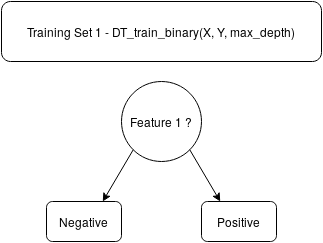
\includegraphics[scale=0.75]{Train1.png}
    
    \noindent Accuracy = 0.75
    
\end{center}

\begin{center}
    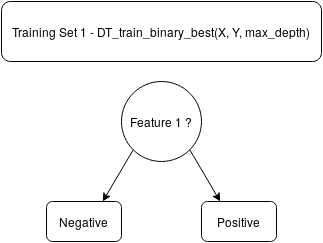
\includegraphics[scale=.75]{Train1best.png}
    
    \noindent Accuracy = 0.75
     
\end{center}

\noindent \textbf{Training Set 2 Results}

\indent The same two training functions were also run on Training Set 2. With "max\textunderscore depth" set to -1, "DT\textunderscore train\textunderscore binary(X, Y, max\textunderscore depth)" produces a model with an accuracy of 1.0. "DT\textunderscore train\textunderscore binary\textunderscore best(X\textunderscore train, Y\textunderscore train, X\textunderscore val, Y\textunderscore val)" also produces a model with an accuracy value of 1. However, if the "max\textunderscore depth" is set to 1 produces a model with an accuracy value of 0.66 on the test data. This is another case where limiting the "max\textunderscore depth" reduces the accuracy of the model. If overfitting is a problem, limiting "max\textunderscore depth" is an option for improving results but limiting it too much leads to underfitting. 

\begin{center}
    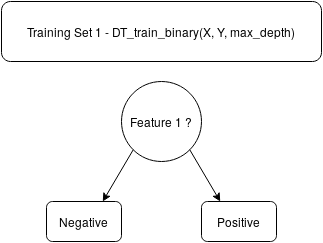
\includegraphics[scale=0.75]{Train1.png}
    
    \noindent Accuracy = 1.0
    
\end{center}

\begin{center}
    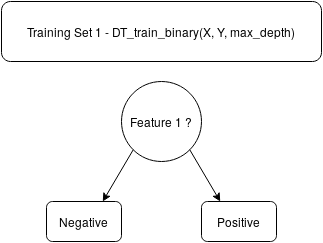
\includegraphics[scale=0.75]{Train1.png}
    
    \noindent Accuracy = 1.0
    
\end{center}

\section*{4. On Inviting Friends for Dinner}

\indent Three decision trees were trained based on three different subsets of samples regarding whether or not to invite friends for dinner. The first subset of samples consisted of samples 1 through 5, the second subset consisted of samples 3 through 7, and the last subset consisted of samples 4 through 8. The accuracy of the first tree when tested against the three test samples was 0.333. The same accuracy was yielded when testing the second subset. Testing the last subset of data yielded and accuracy of 0.666. The predictions for the first and second of those samples was a unanimous yes. When predicting the outcome of the third sample, however, the final tree predicted no, which is correct, but the vote on the prediction of the third sample still resulted in a positive prediction. The vote in this 

\begin{center}
    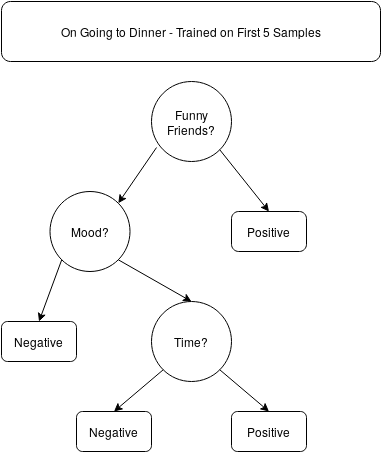
\includegraphics[scale=0.65]{First.png}
    
    \noindent Accuracy = 0.333
    
\end{center}

\begin{center}
    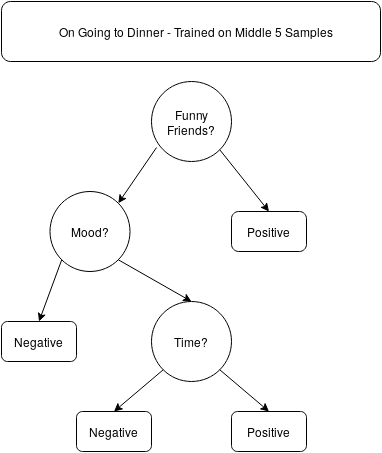
\includegraphics[scale=0.65]{Middle.png}
    
    \noindent Accuracy = 0.333
    
\end{center}

\begin{center}
    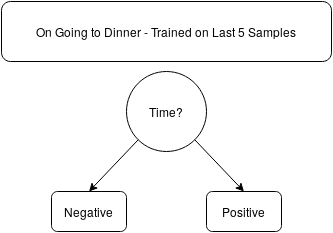
\includegraphics[scale=0.75]{Last.png}
    
    \noindent Accuracy = 0.666
    
\end{center}

\section*{5. On Building Decision Trees from Real-Valued Data}

\indent One decision tree was trained based on real-valued data. This was done by calling "DT\textunderscore train\textunderscore real(X, Y, max\textunderscore depth)". Using a "max\textunderscore depth" value of -1 yields the decision tree below with an accuracy value of 1.0. Another decision tree was generated using "DT\textunderscore train\textunderscore binary\textunderscore best(X\textunderscore train, Y\textunderscore train, X\textunderscore val, Y\textunderscore val)". It produced the same tree and same accuracy value.

\begin{center}
    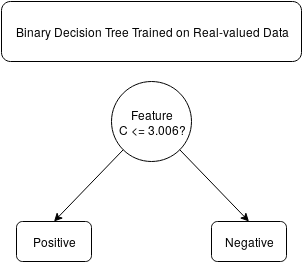
\includegraphics[scale=0.75]{real.png}
    \newline \newline Accuracy = 1.0
\end{center}

\end{document}





















